\documentclass[12pt]{article}
\usepackage{amsmath}
\usepackage{graphicx}
\usepackage{pdfpages}
\usepackage{amssymb}
\usepackage{float}

\title{Exercise Set 9}
\author{Ryan C. Bleile}

\begin{document}
\maketitle
\newpage

\section*{Discrete Heat Diffusion}

We will begin our discussion with the 1-D heat diffusion equation: 

\[ \frac{\partial u(x,t)}{\partial t} = \frac{\partial}{\partial t}(k(x) \frac{\partial u(x,t)}{\partial x}) \] 

Here u(x,t) describes the temperature at any given point and time. And K(x) is the measure of how the material diffuses heat at any given point along the object. In order to simplify the solution to this P.D.E. we will establish the boundary conditions that u(-$\pi$, t) = u($\pi$, t), these boundary conditions describe the scenario of a closed loop system.

\subsection*{Discretization}

\ \ \ In order to solve this PDE using Linear Algebra methods it is important that we first discretize the PDE into a system of ODE, which we are then able to solve via Linear Algebra techniques. In order to solve this as an ODE we wish to have the above equation fit the form:

\[ \frac{du}{dt} = Au  \]

for it is this equation which we know how to solve. Looking at our above example we will begin by using calculus and algebra to simplify he expression into pieces we are able to work with.

\begin{eqnarray*}
\frac{\partial u(x,t)}{\partial t} &=& \frac{\partial}{\partial t}(k(x) \frac{\partial u(x,t)}{\partial x})\\
&& CHAIN\ RULE\\
\frac{\partial u(x,t)}{\partial t} &=& \frac{\partial k(x)}{\partial x}\frac{\partial u(x,t)}{\partial x}+k(x)\frac{\partial^2 u(x,t)}{\partial x^2}
\end{eqnarray*}

In this example we will look at the case when k(x) = x. This leads to:

\begin{eqnarray*}
\frac{\partial u(x,t)}{\partial t} &=& \frac{\partial u(x,t)}{\partial x}+ x\frac{\partial^2 u(x,t)}{\partial x^2}
\end{eqnarray*}

If we now move from the continuous to the discrete case x becomes $\vec{x}$ and our derivatives can be rewritten as matrix operators. Looking first at our simple 1$^{st}$ derivative we can see that there are 3 ways in which to calculate the derivative, the left-side, right-side, or mid-point approximation. These three approximations can be calculated in this manner:

\begin{eqnarray*}
right &=& \frac{X_{n+1} - X_{n}}{\Delta X}\\
left &=& \frac{X_{n} - X_{n-1}}{\Delta X}\\
mid-Point &=& \frac{X_{n+1} - X_{n-1}}{2 \Delta X}
\end{eqnarray*}

Using this we can discretize the derivative by finding a matrix which will produce this result when multiplied by the vector $\vec{x}$. For these three derivatives these matrices can be formed:

\[
right = \frac{1}{\Delta X}
\begin{bmatrix}
-1 & 1 & 0 &  ... & 0\\
0 & -1 & 1 & 0 &  ...\\
& & ... & & \\
1 & 0 & ... & 0 & -1
\end{bmatrix}
\]
\[
left = \frac{1}{\Delta X}
\begin{bmatrix}
1 & 0 & 0 &  ... & -1\\
-1 & 1 & 0 & 0 &  ...\\
& & ... & & \\
0 & 0 & ... & -1 & 1
\end{bmatrix}
\]
\[
Mid-Point = \frac{1}{2 \Delta X}
\begin{bmatrix}
0 & 1 & 0 &  ... & -1\\
-1 & 0 & 1 & 0 &  ...\\
& & ... & & \\
1 & 0 & ... & -1 & 0
\end{bmatrix}
\]

Since none of these first derivatives are symmetric there is no obvious choice as of right now as of which is the best to use for our approximation. It is interesting to not however that the mid-Point derivative the matrix is anti-symmetric.

Next we will discretize the second derivative. This derivative can be found in a symmetric fashion where we use the left and right hand derivatives combined to give us our symmetric second derivative. the second derivative can be written down as;

\begin{eqnarray*}
\frac{d^2 f}{dx^2}(x_{n}) &=& \frac{(f_{n+1} - f_{n}) - (f_{n} - f_{n-1})}{(\Delta X)^2}\\
\\
&=& \frac{f_{n+1} - 2f_{n} + f_{n-1}}{(\Delta X)^{2}}
\end{eqnarray*}

which can be written as this matrix:

\[
Second-Deriv = \frac{1}{(\Delta X)^{2}}
\begin{bmatrix}
-2 & 1 & 0 & 0 & ... & 1\\
1 & -2 & 1 & 0 & ... & 0\\
0 & 1 & -2 & 1 & ... & 0\\
  &   & ...&...&     &  \\
1 & ... & 0 & 0 & 1 & -2   
\end{bmatrix}
\]

This is not the end of the story however since the second derivative is also multiplied with the scaling factor x.Where x will be N for the case of discritization, meaning that each row is multiplied by the row number. this can be added to our matrix such that:

\[
x\frac{d^{2}}{dx^{2}} = \frac{1}{(\Delta X)^{2}}
\begin{bmatrix}
-2 & 1 & 0 & 0 & ... & 1\\
2 & -4 & 2 & 0 & ... & 0\\
0 & 3 & -6 & 3 & ... & 0\\
  &   & ...&...&     &  \\
N & ... & 0 & 0 & N & -2N 
\end{bmatrix}
\]

If we call the first derivative matrix A and the x times the second derivative matrix B we have reduced our continuous expression for x and t into one that is continuous in time but discrete in x as follows.

\begin{eqnarray*}
\frac{d \vec{u}}{dt} &=&  \textbf{A}\vec{u} + \textbf{B}\vec{u}\\
&=&(\textbf{A}+\textbf{B})\vec{u}
\end{eqnarray*}

Which means we can combine our matrices into one simple expression:

\begin{eqnarray*}
\frac{d \vec{u}}{dt} &=& \textbf{C} \vec{u}
\end{eqnarray*}

where C = A+B.

Now that we have a system that is in the form we wished, it is important for us to analyze the matrix we developed as our diffusion operator. So we will now take a closer look at our matrix C.

\subsection*{Studying our Discrete Matrix}

\ \ \ We will analyze this matrix in MatLab in order to determine a number of its features. First however we notice that the matrix is not symmetric. This means that there is a very high probability that there will be complex eigenvalues, and in fact there is. Our goal for this study is to determine six eigenvalues which are the closest to zero. we can do this by taking the absolute value of the complex conjugates of every eigenvalue. This operation will give us a list of eigenvalues from 0 to some positive number. We can than take this list and pull off the eigenvalues associated with the six lowest terms in this set and plot their eigenvectors. Following is the MatLab code used to analyze this matrix:

\begin{verbatim}
N = 100;
X = linspace(-pi, pi, N);
dx = X(2) - X(1);

A = zeros([N N]);

for jndex = 1:N
    for index = 1:N
        if (jndex == index)
            A(index, jndex) = -2*X(index);
        elseif (jndex+1 == index || jndex-1 == index)
            A(index, jndex) = X(index);
        end
    end
end

B1 = toeplitz([-1 1 zeros(1, N-2)] )/dx;
B2 = toeplitz( [1 zeros(1, N-2) -1] )/dx;
B3 = toeplitz( [0 1 zeros(1, N-3) -1] )/dx;

C1 = A+B1;
C2 = A+B2;
C3 = A+B3;

[V1,D1] = eigs(C1,98,'sm');
[V2,D2] = eigs(C2,98,'sm');
[V3,D3] = eigs(C3,98,'sm');

figure
for i=1:98
    plot(V1(:,i));
    pause(.1);
end
pause(1);
for i=1:98
    plot(V2(:,i));
    pause(.1);
end
pause(1);
for i=1:98
    plot(V3(:,i));
    pause(.1);
end
\end{verbatim}

This code was used to find the magnitudes of the eigenvalues, ordered from smallest to largest for our three different scenarios and than just for a picture it plots a quick animation cycling through each eigenvector associated with ordered list of eigenvalues. Some interesting patterns emerge and a few of these eigenvector plots will be shown below. Starting with our most standard derivative, the right handed derivative from which our definition of the derivative stems we see that the values closest to zero give us fairly even steady sine and cosine terms. As we increase to larger eigenvalues these functions take on a lot of randomness and are not even across the domain.\\ 

Plotting the other two derivative sets as well reveals some interesting results. Firstly, the second set of eigenvectors yields results that start with the highest amount of randomness and noise in the lowest eigenvectors and the most ordered states are those from the highest eigenvalues. But these more ordered terms do not fit sine or cosine in the same nice form that set one gave.\\

The third set contains some of the most interesting eigenvectors. Just as a reminder, the third set is fro the anti-symmetric first derivative. This set contains a large number of circular eigenvectors. and bounces back and forth between random wave pattern and circular patterns tending towards circular patterns as the eigenvalues increase in magnitude and finally settling to a few nearly perfect circles. and then even into a few beautiful sin or cosine curves.\\

\subsubsection*{Eigenvectors for the First Matrix}
\begin{figure}[H]
	\begin{minipage}[b]{0.5\linewidth}
	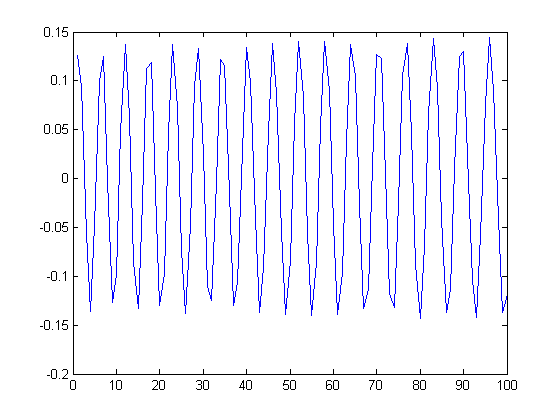
\includegraphics[scale=.5]{v1p1.png}
	\caption{EigenVector 1}
	\end{minipage}
	\begin{minipage}[b]{0.5\linewidth}
	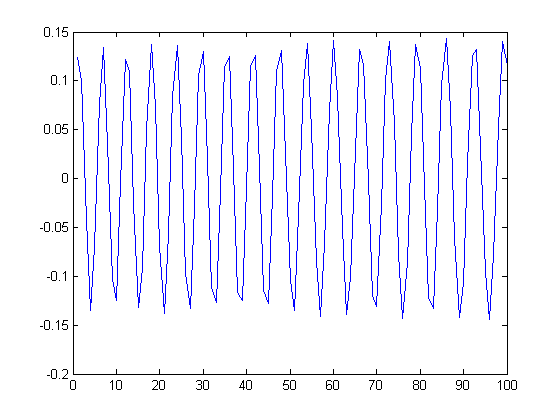
\includegraphics[scale=.5]{v1p2.png}
	\caption{EigenVector 2}
	\end{minipage}
\end{figure}

\begin{figure}[H]
\begin{minipage}[b]{0.5\linewidth}
	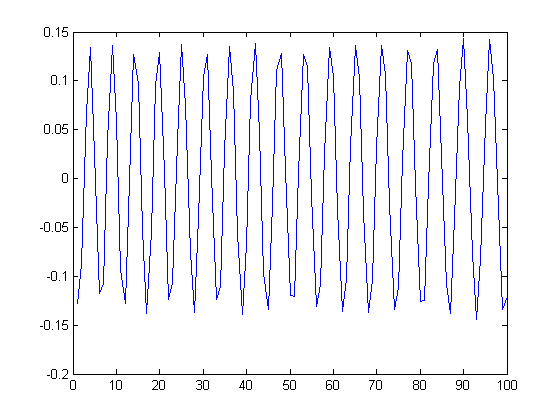
\includegraphics[scale=.5]{v1p3.png}
	\caption{EigenVector 3}
\end{minipage}
\begin{minipage}[b]{0.5\linewidth}
	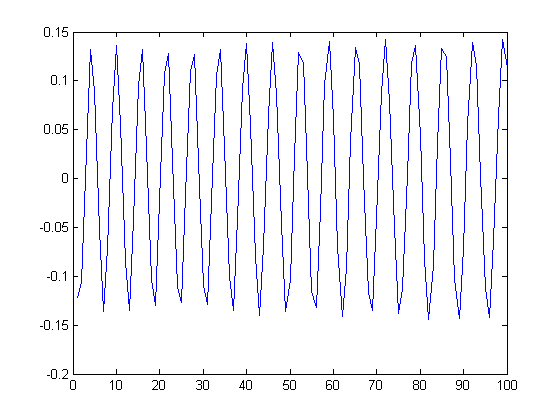
\includegraphics[scale=.5]{v1p4.png}
	\caption{EigenVector 4}
\end{minipage}
\end{figure}

\begin{figure}[H]
\begin{minipage}[b]{0.5\linewidth}
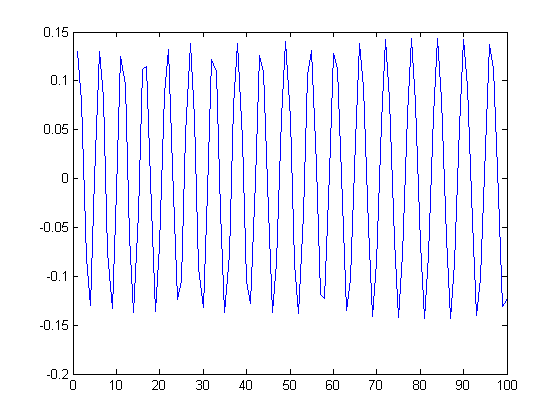
\includegraphics[scale=.5]{v1p5.png}
\caption{EigenVector 5}
\end{minipage}
\begin{minipage}[b]{0.5\linewidth}
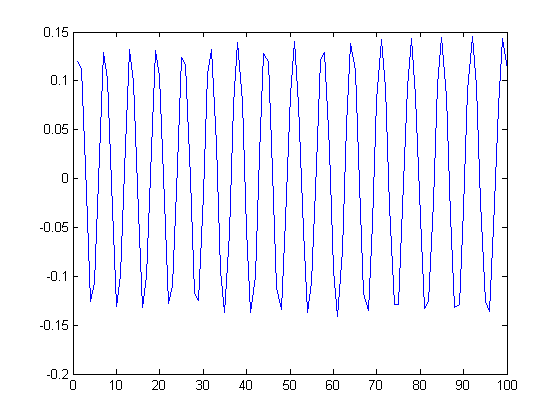
\includegraphics[scale=.5]{v1p6.png}
\caption{EigenVector 6}
\end{minipage}
\end{figure}


\subsubsection*{Eigenvectors for the Second Matrix}


\begin{figure}[H]
\begin{minipage}[b]{0.5\linewidth}
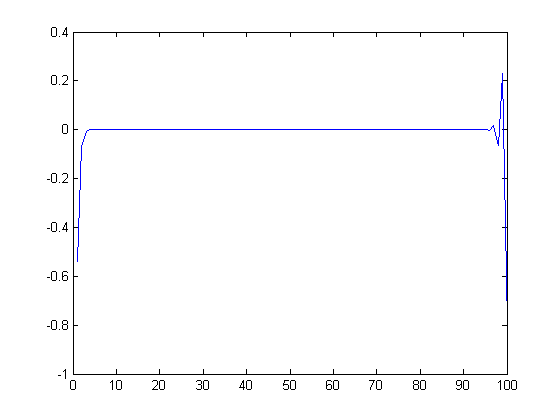
\includegraphics[scale=.5]{v2p1.png}
\caption{EigenVector 1}
\end{minipage}
\begin{minipage}[b]{0.5\linewidth}
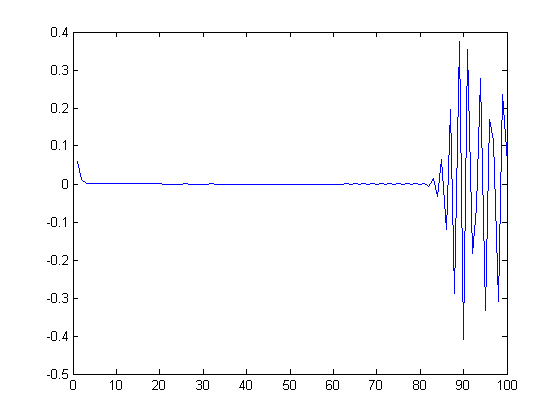
\includegraphics[scale=.5]{v2p4.png}
\caption{EigenVector 4}
\end{minipage}
\end{figure}

\begin{figure}[H]
\begin{minipage}[b]{0.5\linewidth}
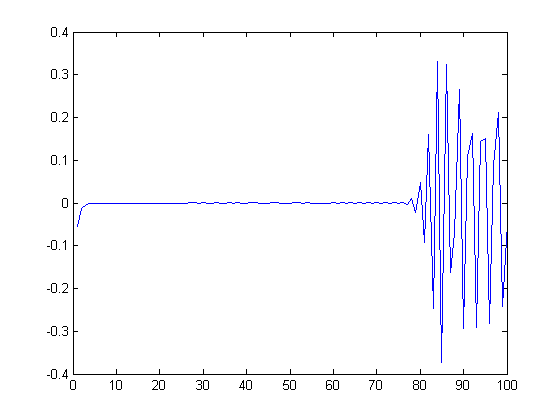
\includegraphics[scale=.5]{v2p6.png}
\caption{EigenVector 6}
\end{minipage}
\begin{minipage}[b]{0.5\linewidth}
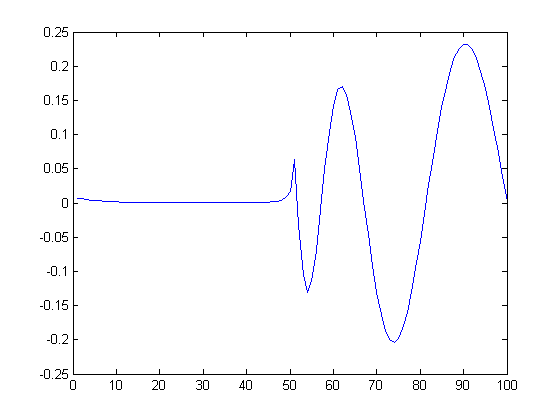
\includegraphics[scale=.5]{v2p90.png}
\caption{EigenVector 90}
\end{minipage}
\end{figure}

\subsection*{Eigenvectors for the Third Matrix}

\begin{figure}[H]
\begin{minipage}[b]{0.5\linewidth}
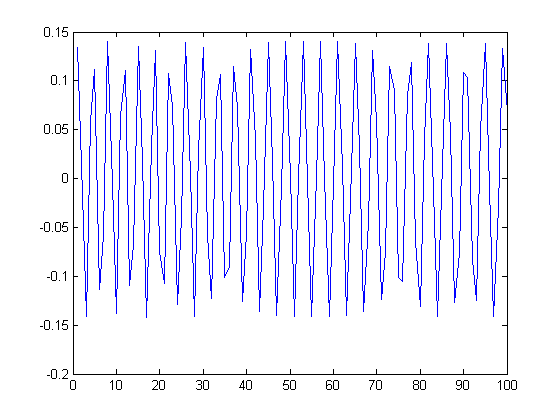
\includegraphics[scale=.5]{v3p1.png}
\caption{EigenVector 1}
\end{minipage}
\begin{minipage}[b]{0.5\linewidth}
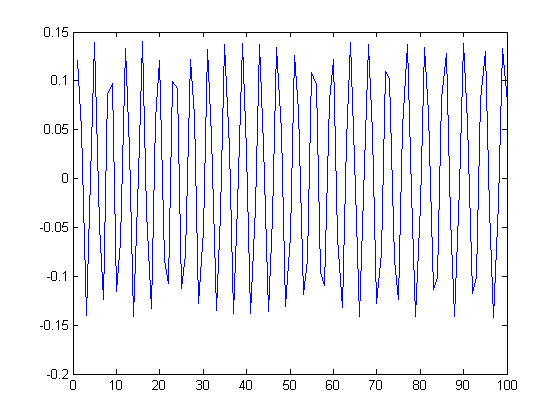
\includegraphics[scale=.5]{v3p4.png}
\caption{EigenVector 4}
\end{minipage}
\end{figure}

\begin{figure}[H]
\begin{minipage}[b]{0.5\linewidth}
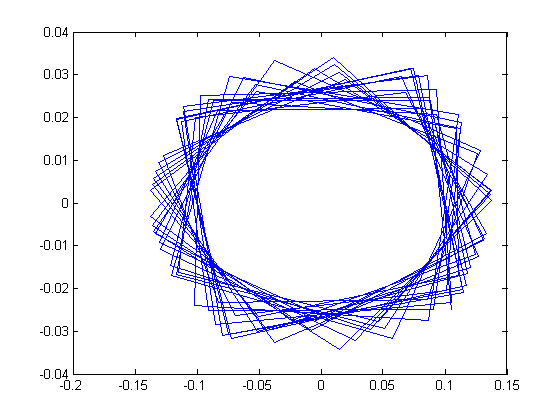
\includegraphics[scale=.5]{v3p11.png}
\caption{EigenVector 11}
\end{minipage}
\begin{minipage}[b]{0.5\linewidth}
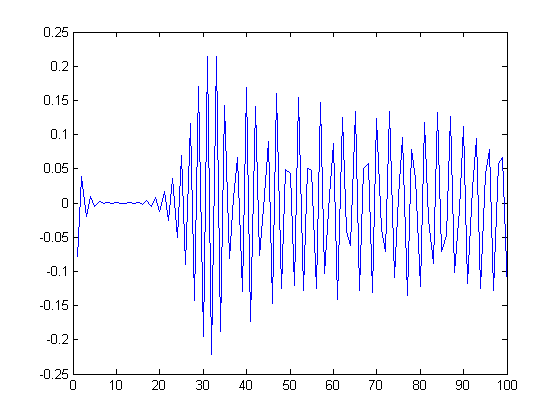
\includegraphics[scale=.5]{v3p50.png}
\caption{EigenVector 50}
\end{minipage}
\end{figure}

\begin{figure}[H]
\begin{minipage}[b]{0.5\linewidth}
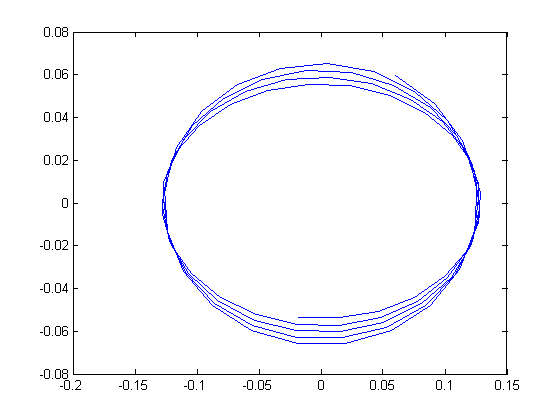
\includegraphics[scale=.5]{v3p90.png}
\caption{EigenVector 90}
\end{minipage}
\begin{minipage}[b]{0.5\linewidth}
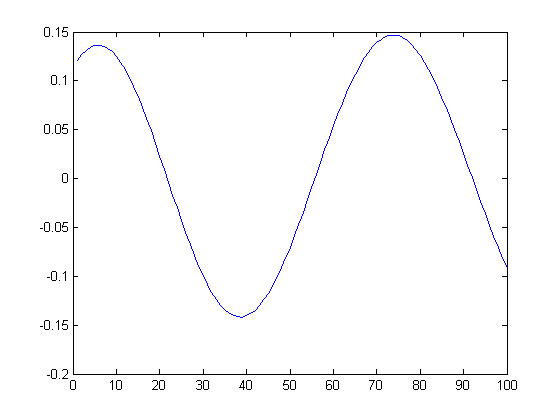
\includegraphics[scale=.5]{v3p97.png}
\caption{EigenVector 97}
\end{minipage}
\end{figure}

\subsection*{Conclusion}

For a full view of the eigenvalues, those from 1 to 98 out of 100 total, which are the only ones eigs() can return for complex valued matrices, run the sample matlab code and view the animation. I have a great deal of personal interest in the differences between these and how they would be used to solve the heat equation. Also how do the differences in these methods change the solution for the discritized case. And lastly do all of these ways converge to the same result as the size of N increases, i.e. do all of these methods converge to the same continuous limit. These are all questions worth exploring but are outside of the bounds of the time line for this assignment.

\end{document}
